\documentclass[10pt,a4paper,basque]{article}
\usepackage[T1]{fontenc}
\usepackage[utf8]{inputenc}
\usepackage[basque]{babel}
\usepackage[parfill]{parskip}
\usepackage{listings}
\usepackage{graphicx}

\graphicspath{{plots/}}
\lstset{language=C, breaklines=true, tabsize=4,showstringspaces=false}
\author{Jon Ezeiza}
\title{FindRoot funtzioaren inplementazioa}
\begin{document}

\maketitle

\begin{abstract}
$f: R^n \rightarrow R^n$ formako funtzioen erroak kalkulatzen dituen programa bat inplementatzea da praktika honen helburua. Hau konputazioko problema klasiko bat da eta FindRoot izena eman ohi zaie funtzioa hau betetzen duten programei.

Erroaren kalkulua hurbilketaz egiten da, Newton-Raphson metodo iteratiboa erabiliz hain zuzen. Ekuazio sistemak ebazteko metodo aljebraiko klasikoak ez dira nahiko flexibleak, ez baitako metodo bakarra $R^n \rightarrow R^n$ domeinu osoa lantzea ahalbidetzen duena. Gainera, metodo eta algoritmo guzti horiek konputazioak eskuz egiteko daude diseinatuta eta, ondorioz, ez dira aukera hoberena konputagailu batean inplementatzeko.

Gaur egungo sistemek duten konputazio ahalmena kontuan harturik, hurbilpen iteratiboa da dudarik gabe aukera egokiena kasuistika gehienetarako. Esan bezala, jada badugu metodo sinple bat, Newton-Raphson metodoa, edozein ordenatako funtzioen erroa hurbildu dezakeena nahi adinako zehaztasunarekin eta eraginkortasun handiarekin. 
\end{abstract}

\section{Oinarri teorikoak}
FindRoot funtzioa jada denbora luzez ezagunak izan diren kontzeptu matematikoetan dago oinarrituta. Atal honetan oinarri teoriko horiek laburki azalduko dira, programaren inplementazioan hartu diren erabakiak zein kontzeptutan oinarritzen diren zehazteko.

\subsection{Taylor-en garapena}

Taylor-en garapenari esker, edozein funtzio jarraitu bere deribatuen konbinazio lineal bidez adieraz daiteke, funtzioak puntu jakin batean duen balioa emanda. Funtzioa $n$ aldiz deribagarria bada konputatu nahi dugun puntuan, zehaztasun osoz adierazi ahalko da serie infinitu baten bitartez.

Hala ere, funtzio guztiek ez dute baldintza hori betetzen, eta konputazioaren arloan ez da fisikoki posiblea serie infinituak kalkulatzea. Taylor-en garapena, ordea, funtzioaren balioa hurbiltzeko ere erabili daiteke. Geroz eta deribatu gehiago erabili, orduan eta zehatzagoa izango da hurbilpena emandako hasierako balioa egokia bada. Horrez gain, Taylor-en garapenak  hurbilpenaren errorea bornatzeko ahalmena ere ematen digu.

$$f(x + h) = \sum_{n = 0}^{\infty} \frac{1}{n!} f^{(n)}(x) \cdot h^n$$

$$f(x + h) = (\sum_{n = 0}^{k} \frac{1}{n!} f^{(n)}(x) \cdot h^n) + \frac{1}{(k+1)!} f^{(k+1)}(c) \cdot h^{k+1} \quad non \quad c \in (x, x+h)$$

\subsection{Newton-Raphson metodoa}

Taylor-en garapena oso erabilgarria izan daiteke zenbait kontextutan, hala ere, praktika hau lantzeko momentuan ez daukagu ezagutza nahikorik funtzio baten deribatuak automatikoki kalkulatzeko eta ez da arrazoizkoa jakobiar guztiak erabiltzaileari eskatzea kasu bakoitzean. Hortaz, metodoaren moldapen bat behar dugu, deribatuak era sistematikoan kalkulatzea behar ez duena, Newton-Raphson metodoa hain zuzen.

Newton-Raphson metodoa da FindRoot funtzioaren muina. Metodo honek Taylor-en lehenengo mailako garapena erabiltzen du soilik funtzioaren erroa hurbiltzeko. Deribatu segida luze bat batu beharrean, hasierako balioarekin hasiz, behin eta berriro pasako du formula sinple batetik, iterazio bakoitzean helburura gehiago hurbiltzen delarik. Hortaz, emaitzaren zehaztasuna iterazio kopuruaren mendekoa da, eskura ditugun deribatu kopuruaren mendekoa izan beharrean. Hau askoz maneiagarriagoa konputazioaren ikuspegitik.

Horrez gain, emaitza baten errorea bornatu daiteke. Errore maximoa beti iterazio bateko eta aurreko iterazioko emaitzen arteko diferentziaren norma izango da.

Aipatutako formula, ezan bezala, Taylor-en lehen mailako garapenetik lor daiteke zuzenean.

$$0 = f(x) \cong f(x_0) + f'(x_0) \cdot (x - x_0)$$

$$x = x_0 - \frac{f(x_0)}{f'(x_0)}$$

$n$ dimentsiotan honela geldituko litzateke.

$$\bar{x} = \bar{x_0} - j(\overline{x_0})^{-1} \cdot f(\overline{x_0})$$

$$
\left(
\begin{array}{c}
x_1\\
x_2\\
\vdots\\
x_n
\end{array}
\right) = 
\left(
\begin{array}{c}
x_{0_1}\\
x_{0_2}\\
\vdots\\
x_{0_n}
\end{array}
\right) -
\left(
\begin{array}{cccc}
\frac{\partial f_{1}(\overline{x_0})}{\partial \overline{{x_0}_1}} & \frac{\partial f_{1}(\overline{x_0})}{\partial \overline{{x_0}_2}} & \ldots & \frac{\partial f_{1}(\overline{x_0})}{\partial \overline{{x_0}_n}}\\
\frac{\partial f_{2}(\overline{x_0})}{\partial \overline{{x_0}_1}} & \frac{\partial f_{2}(\overline{x_0})}{\partial \overline{{x_0}_2}} & \ldots & \frac{\partial f_{2}(\overline{x_0})}{\partial \overline{{x_0}_n}}\\
\vdots & \vdots &  & \vdots\\
\frac{\partial f_{n}(\overline{x_0})}{\partial \overline{{x_0}_1}} & \frac{\partial f_{n}(\overline{x_0})}{\partial \overline{{x_0}_2}} & \ldots & \frac{\partial f_{n}(\overline{x_0})}{\partial \overline{{x_0}_n}}
\end{array}
\right)^{-1} \cdot
\left(
\begin{array}{c}
f_{1}(\overline{x_0})\\
f_{2}(\overline{x_0})\\
\vdots\\
f_{n}(\overline{x_0})
\end{array}
\right)
$$

Iterazio bakoitzeko errore maximoa $|j(\overline{x_0})^{-1} \cdot f(\overline{x_0})|$ izango da beraz.

\subsubsection{Konbergentzia lokalaren teorema}

Taylor-en garapenetik lortu denez, badakigu Newton-Raphson-en lehenengo iterazioaren emaitza emandako hasierako puntua baina gertuago egongo dela funtzioaren errotik. Hala ere, honek ez du frogatzen sekuentziak beti helburuan konbergituko duenik.

Konbergentzia lokalaren teoremari esker, badakigu behintzat $\forall x \in (x_0, x): \quad |x_0 - j(\overline{x_0})^{-1} \cdot f(\overline{x_0})| < 1$ espresioa betetzen bada, $x_0$ horrekin Newton-Raphson sekuentziak $x$ errorantz konbergituko duela. Hau honela da $x$ erroa Newton-Raphson formularen puntu finkoa delako.

Hona hemen konbergentzia lokalaren teoremaren adierazpen formala.

Izan bitez $g:R^n \rightarrow R^n$ funtzioa, honen $p$ puntu finkoa, $g(p) = p$ izanik, eta $x_i = g(x_{i-1}) \quad i = 1, 2, ..., n$ sekuentzia.

Izan bedi, gainera, $T_{\delta} = (p - \delta, p + \delta)$ tartea, $\forall x \in T_{\delta} \quad |g(x)| < 1$ izanik.

Baldin, $x_0 \in T_{\delta}$, honako hauek beteko dira.

\begin{itemize}
\item $x_i \in T_{\delta} \quad i = 1, 2, ..., n$
\item $\lim_{n \rightarrow \infty} x_i = p$
\item $\neg\exists q \in T_{\delta} : \quad q \neq p \wedge g(q) = q$
\end{itemize}

\subsubsection{Arazoak}

Konbergentzia lokalaren teoremak exekuzio egokia ziurtatzen digu zenbait baldintza konkretutan. Baldintza horietatik kanpo ere emaitza zuzenera konbergitzea ere posible da, baina ez dago ziurtatuta.

FindRoot programa arazo anitzekin aurki daiteke, problema ebazteko hasierako puntu desegokia eman delako edo emandako funtzioaren izaera intrintsekoagatik.

Hona hemen arazo esanguratsuenak.

\paragraph{Jakobiar nulua edo singularra}

Jakobiar guztiak ez dira beti alderantzikagarriak edo deskonposagarriak. Hortaz, kasu horietan ezingo da $j(\bar{x}) * \delta \bar{x} = f(\bar{x})$ ekuazio sistema ebatzi eta Newton-Raphson metodoak ezingo du jarraitu.

\paragraph{Dibergentziak}

Esan bezala, Newton-Raphson metodoak ez du beti konbergitzen, funtzioaren izaeraren eta hasierako puntuaren araberakoa da. Zenbait kasutan algoritmoak dibergituko du konbergentzia zona batera iritsi baino lehen, eta beste batzuetan betirako jarraituko du dibergitzen.

\paragraph{Singularitateak eta puntu ez deribagarriak}

Funtzio guztiak ez dira deribagarriak puntu guztietan, hortaz, batzuetan Newton-Raphson metodoa erabiltzean jarraitu ezin den puntu batera irits daiteke. Gainera, singularitateek ere arazoak ekar ditzakete. Zenbait singularitatek algoritmoa erakarriko dute, zenbaitek kontrakoa egingo dute.

\paragraph{Begizta amaigabeak}

Algoritmoak konbergitzen ari denean ere, ez da ziurra puntu zehatz batean amaituko duenik. Batzuetan, funtzioaren izaeragatik edo konputazio erroreengatik, algoritmoa begizta infinitu batean sartu daiteke.

\section{Programaren erabilera}

Inplementatutako programak, oinarrian, ematen zaion funtzioaren erroa aurkitzen du. Hala ere, praktikan, problema dirudiena baina konplexuagoa da.

Funtzioaz gain, funtzioaren lehen mailako jakobiarra eman beharko da. Gainera, programari hasierako puntu bat eman beharko zaio prozesua hasteko. Programak ematen duen emaitza hurbilpen bat izango da, beraz, errore edo tolerantzia maximo bat ere eman beharko da, ez baitu ia inoiz emaitza guztiz zuzena emango.

Emaitzaren zehaztasuna faktore askoren araberakoa da, esaterako, funtzioaren izarak eta hasierako puntuak eragin handia dute. Arazoak maiz gertatuko dira, programak emaitza konkretu batera iritsi gabe infinituraino dibergitzen jarraitzen duelako, begizta itxi batean sartzen delako, puntu berezi batera iritsi eta jarraitu ezin duelako... Kasu askotan, arazo hauek ekiditea ez dago inplementatzailearen eskuetan, sarrera datuen araberakoak izaten baitira. Newton-Raphson metodoak ez du beti emaitza egoki bat ematen, erabiltzailearen ardura da metodoaren izaera ezagutzea eta, adibidez, hasierako puntu egokiak aukeratzea emaitza bermatzeko.

Dena den, programak ondo erantzun behar du kasu guztietan. Ahalik eta informazio gehien eman behar zaio erabiltzaileari lortutako emaitzak ondo interpreta ditzan. Arazo bat aurkitzean, ondo azaldu behar zaio erabiltzaileari zer den zehazki gaizki joan dena, sarrera datuak aldatzeko erabakia errazteko eta problema era desberdin batean ebatzi ahal izateko. Azkenik, arazo hauei aurre egiteko eta prozesuarengan ahalik eta kontrol handiena izateko aukera nahikoak eman behar ditu programak.

Programa eraikitzean faktore guzti hauek hartu dira kontuan. Hona hemen, inplementazio hau erabiltzeko gida, non programaren aukera guztiak deskribatzen diren eta emaitzak nola interpretatu zehazten den.

\subsubsection{Konpilazioa}

Programa erraz konpilatzeko \emph{Makefile} bat gehitu da. Hortaz, \emph{make} programa erabiltzea nahikoa da exekutagarria lortzeko. Programaren zatiak independenteki konpilatzeko ere aukera ematen du \emph{Makefile}-ak.

\begin{itemize}
\item \emph{make} programa osoa konpilatzeko.
\item \emph{make findroot.o} programa nagusia soilik konpilatzeko.
\item \emph{make function.o} prozesatu beharreko funtzioa soilik konpilatzeko.
\item \emph{make norm.o} ordezko norma soilik konpilatzeko.
\item \emph{make clean} konpilazioan sortutako fitxategiak ezabatzeko.
\end{itemize}

Honetarako, ordea \emph{make} programa eta \emph{GSL} liburutegia instalatuta eduki behar dira.

\emph{GSL} aparte konpilatuta badago, honela konpilatu daiteke programa hau.

\begin{lstlisting}
gcc -Wall findroot.c function.c norm.c -o findroot -lgsl -lgslcblas -lm -O2 -I<a> -L<b>
\end{lstlisting}

\begin{itemize}
\item <a>: GSL liburutegi konpilatuaren \emph{include} direktorioaren path absolutua.
\item <b>: GSL liburutegi konpilatuaren \emph{lib} direktorioaren path absolutua.
\end{itemize}

\subsubsection{Exekuzioa}

Behin konpilazioa bukatuta, lortutako exekutagarriari deitzea nahikoa izango da programa hasteko. Programa parametrorik gabe exekutatzen bada, errore mezu bat agertuko da konfigurazio fitxategiaren izena pasa behar zaiola esanez. Exekutagarriak berak, ez du parametro gehiagorik hartzen, sarrera datu guztiak konfigurazio fitxategitik irakurriko baititu.

\begin{lstlisting}
.\findroot config.txt
\end{lstlisting}

Emaitzak irteera estandarrean inprimatuko dira. Dena ondo joan bada, erroaren hurbilpenaz gain, erroaren errore maximoa, erroaren irudia emandako funtzioarekiko, iterazio kopurua eta Newton-Raphson metodoa bera exekutatzen eman den denbora, begiztaren exekuzioarena soilik, itzuliko dira.

\subsubsection{Konfigurazio fitxategia}

Funtzioa eta jakobiarra objektu fitxategi moduan pasatzen zaizkio programari konpilazioaren \emph{linking} fasean. Beste datu guztiak exekuzio garaian irakurriko dira konfigurazio fitxategi honetatik.

Emandako funtzioen eta hasierako puntuaren dimentsioa zehaztea ezinbestekoa da, hori izango da beraz, konfigurazio fitxategian emango den lehen datua. Dimentsioak, noski, zenbaki arrunta izango da, eta zero baina handiagoa izan beharko du. Ondoren, dimentsioa jakinda, hasierako puntuaren elementuak zerrendatuko dira, elementu bakoitza koma higikorreko zenbaki batekin adierazita.

Datu hauek soilik ematea nahikoa da programa era normalean erabiltzeko. Hala ere, inplementazio honek aukera asko ematen ditu prozesua nahi bezala kontrolatzeko. Ezer espezifikatu ezean, aukera hauei balio lehenetsiak esleituko zaizkie; baina, nahi izanez gero, konfigurazio fitxategi honetan ordezko balioak zehaztu daitezke dimentsioa eta hasierako puntua eman ondoren.

Hona hemen fitxategiak izan behar duen sintaxia.

\begin{verbatim}
dimentsioa n
X1
X2
...
Xn
<aukera_izena> <balioa>
...
\end{verbatim}

Lerro hutsak eta \emph{\#} karakterearekin hasten diren lerro guztiak ez dira kontuan hartuko. Gainera, inplementazioaren izaeragatik, sintaxi egokiko lerro baten ondoren edozer jartzea onartzen da, lerro berean dagoen bitartean. Programak bakarrik lerroaren balizko hasiera hartuko du kontuan. Dena den, gomendagarria da ezer gehigarririk ez jartzea.

\subsubsection{Aukerak}

\paragraph{Tolerantzia}

Tolerantziak emaitza egokitzat ematen den erroaren errorea bornatzen du. Newton-Raphson metodoaren iterazio bakoitzean, esan bezala, konbergentzia zona batean egotekotan, emaitzaren errorea jaitsiz joango da era koadratikoan. Hortaz, iterazio mugara iristen ez den bitartean, programak iteratzen jarraituko du emaitzaren errorea tolerantzia baina txikiagoa den arte. Prozesua ez da geldituko konbergentzia eremu batean ez badago ere, iteratzen jarraituko da honelako eremu batean sartuko den esperoan.

Lehenetsitako tolerantzia $10^{-12}$-koa da, eta konfigurazio fitxategian aldatu nahi izanez gero, \emph{tolerantzia} da aukeraren izena. Tolerantzia berri bat definitzen bada, koma higikorreko zenbaki modura adierazi beharko da eta zero baina handiagoa izan beharko du.

Adibidez,

\begin{lstlisting}
...
tolerantzia 1.0e-10
...
\end{lstlisting}

\paragraph{Tolerantzia erlatiboa}

Inplementazio honetan, emaitzaren errorea era absolutuan edo erlatiboan kalkula daiteke. Errore erlatiboa ez da guztiz zehatza izango, errorea iterazio horretako hurbilpenarekin zatitzen baita, amaierako emaitzarekin beharrean. Dena den, praktika hau ere egokia da erabiltzaileak honela egiten dela badaki.

Tolerantzia erlatiboa denean, amaieran inprimatzen den emaitzako errore maximoa ere erlatiboa izango da.

Besterik adierazi ezean, tolerantzia erlatiboa izango da. Aukera honen balioa aldatu daiteke konfigurazio fitxategian \emph{erlatiboa} izenaz. Aukera honek, boolearra izanik, bakarrik \emph{bai} eta \emph{ez} balioak hartuko ditu.

Adibidez,

\begin{lstlisting}
...
erlatiboa ez
...
\end{lstlisting}

\paragraph{Zerorekiko distantzia maximoa}

Tolerantziaz gain, inplementazio honek hurbilpenaren irudiak zerorekiko duen distantzia ere bornatzen du. Programak iteratzen jarraituko du, bai tolerantzia eta bai zerorekiko distantzia maximoaren baldintzak betetzen diren arte.

Lehenetsitako distantzia $10^{-12}$-koa da, eta konfigurazio fitxategian aldatu nahi izanez gero, \verb|max_zero_distantzia| da aukeraren izena. Honen balioak tolerantziarenaren formatu bera du, koma higikorreko zenbakia eta zero baina handiagoa.

Adibidez,

\begin{lstlisting}
...
max_zero_distantzia 1.0e-7
...
\end{lstlisting}

\paragraph{Ordezko norma}

Lehen azaldu den moduan, inplementazio honek, funtzioaren objektu fitxategiaz gain, norma objektu fitxategi bat behar du.

Kontrakoa adierazten ez bada, fitxategi honetako funtzioari ez zaio kasurik egingo, eta BLAS liburutegiak eskaintzen duen norma euklidearra aplikatuko da. Hala ere, erabiltzaileak beste norma bat erabiltzeko aukera du, fitxategi honetan norma funtzio hau definituz.

Aukera hau konfigurazio fitxategian aldatzeko \verb|ordezko_norma| aukera izena erabili beharko da. Hau ere aukera boolearra da, beraz, \emph{bai} eta \emph{ez} balioak onartuko ditu bakarrik.

\begin{lstlisting}
...
ordezko_norma bai
...
\end{lstlisting}

\paragraph{Iterazio kopuru maximoa}
Kasu askotan, emandako funtzioaren eta hasierako puntuaren arabera, programak ez du inoiz konbergentzia zona bat aurkituko eta iteratzen jarraitu lezake gelditu gabe. Hau ekiditeko, iterazio kopuruan muga absolutu bat jarri da.

Lehenetsitako maximoa 25 iteraziokoa da. Konbergentzia zona batean, 10-15 iterazio nahikoa izan ohi dira emaitza onargarri bat lortzeko. Hala ere, balio lehenetsi honek konbergitu baino lehen dibergentzia fase bat egon daitekeela kontuan hartzen du.

Muga aldatu nahi izanez gero, konfigurazio fitxategian \verb|iterazio_maximoa| da aukeraren izena eta balio arrunt positiboak onartuko ditu bakarrik.

Adibidez,

\begin{lstlisting}
...
iterazio_maximoa 20
...
\end{lstlisting}

\paragraph{Iterazio dibergente kopuru maximoa}
Esan bezala, askotan dibergentzia fase bat (errorea handitu txikitu beharrean) izango du algoritmoak konbergitzen hasi baino lehenago. Inplementazio honek fase horrek izan ditzakeen iterazio kopurua murrizteko aukera ere ematen du.

Lehenetsitako balioa 10 iteraziokoa da.

Konfigurazio fitxategian aukerak \verb|dibergentzia_iterazio_maximoa| du izena, eta, oraingoan, zero balioa ere onartzen da, erabiltzaileak zuzenean dibergentzia gertatzen den momentuan programa gelditzeko aukera izan dezan.

Adibidez,

\begin{lstlisting}
...
dibergentzia_iterazio_maximoa 5
...
\end{lstlisting}

\paragraph{Jakobiarraren berrerabilpena}
Newton-Raphson iterazioan gertatzen den eragiketa konputazionalki garestienetakoa LU deskonposaketa da, hots, $j(\bar{x}) * \delta \bar{x} = f(\bar{x})$ ekuazio sistema ebazteko lehenengo pausua. Zorionez, jakina da jakobiarraren deskonposaketa hainbat iteraziotan berrerabili daitekeela konbergentzia prozesua apurtu gabe. Egia da, berez, jakobiarra berrerabiltzeak konbergentzia ordena jaistea dakarrela, iterazio kopurua handitzen baita. Hala ere, kasu gehienetan denbora totala jaisten da, iterazio bakoitza azkarragoa delako.

Ez dago berrerabilpen neurri optimorik kasu guztietarako, dimentsio kopuruaren eta beste faktore batzuen arabera erregulatu behar da. Horregatik, inplementazio honek berrerabilpen ratio hau aldatzea ahalbidetzen dio erabiltzaileari.

Ratio lehenetsia 5 da, hortaz, programak 5 iteraziotan berrerabiliko du jakobiar deskonposatua berri bat kalkulatu baino lehen.

Aukera honen izena \verb|jakobiar_berrerabilpena| da konfigurazio fitxategian, eta zenbaki arruntak onartzen ditu, zero barne.

Adibidez,

\begin{lstlisting}
...
jakobiar_berrerabilpena 2
...
\end{lstlisting}

\subsubsection{Erroreen adierazpena}

Lehenago aipatu den bezala, Newton-Raphson metodoak arazo asko izan ditzake, eta horietako asko ezin dira zuzenean ebatzi beste algoritmo desberdin bat erabili ezean. Kasu horietan, inplementazio honek exekuzioa amaituko du emaitza bat eman gabe.

Dena den, ondoren aipatuko den salbuespen sistemari esker, exekuzio amaitzen duen arazo bat dagoen bakoitzean errore mezu zerrenda bat inprimatzen da ordena hierarkikoan. Lehenengo errore mezuak arazo konkretua deskribatuko du eta ondoren datozenek errore honek programaren hainbat geruzatan izan duen ondorioa erakutsiko dute. Exekuzioa amaitzen duten errore guztiak \verb|[x]| zeinuarekin hasten dira eta errore irteera estandarrean inprimatuko dira.

Azalpen batez gain, zenbait errore mezuk informazio gehigarria dakarte. Hauek \verb|[?]| zeinuarekin hasten dira eta irteera estandarrean inprimatuko dira.

Azkenik, exekuzioa amaitzen ez duten arazoak ere inprimatzen dira, kritikoak ez diren arren, erabiltzaileak gertatu direla jakin beharko lukeelako. Honelako abisu batek, adibidez, programa iterazio mugara iritsi dela eta, ondorioz, emaitza nahi bezain zehatza ez dela esango lezake. Azken mezu hauek \verb|[!]| zeinuarekin hasten dira eta irteera estandarretik inprimatzen dira.

Adibidez, jakobiar singular bat aurkitzen denean, errore mezu hau inprimatuko da.

\begin{lstlisting}
[x] GSL DOMAIN ERROR: matrix is singular
[x] Ezin izan da JX * x = FX ekuazio sistema lineala ebatzi LU deskonposaketa erabiliz.
[?] HURBILPEN PARTZIALA: (-0.5, -0.5)
[?] ERRORE MAXIMOA: 1.79769313486232e+308
[?] F(X): (-0.0792645075960517, -0.14815702328617)
[?] ITERAZIO_KOPURUA: 0
[x] Ezin izan da emaitza kalkulatu.
\end{lstlisting}

\section{Programaren diseinua}

Lantzen ari garen FindRoot algoritmoa problema kritiko bat da konputazioaren munduan. Funtzioen erroak lortzea oinarrizko eragiketa bat da, maiz erabiltzen da eta lortutako emaitzak beste hainbat eragiketa egiteko erabiltzen dira.

Horregatik, garrantzitsua da FindRoot-en inplementazioak arinak, zehatzak eta malguak izatea. Memoria gutxi bete eta exekuzio denbora baxuak izan beharko lituzke. Aldi berean, emaitza ahalik eta zehatzenak eman beharko lituzke eta sarrerako datuen erroreak ahalik eta gutxien maximizatu. Azkenik, funtzio multzo handi baten erroak kalkulatzeko gai izan beharko lirateke, eta aukera anitz eman aipatutako faktoreak nahi bezala balantzatzeko, erabiltzailearen helburuen arabera.

Inplementazio hau printzipio horietan oinarritu da.

Aipatzekoa da kodea iruzkinekin era egokian dokumentatzeko esfortzua egin dela; beti ere ahalik eta iruzkin gutxien idatzita, kodea gehiegi ez lausotzeko. Hala ere, iruzkinak ingelesez idazteko erabakia hartu da, kodearen koherentzia mantentzeko. Praktika honetan garrantzitsua den informazio guztia txosten honetan dago azalduta dena den.

\subsubsection{Newton-Raphson begizta}

Newton-Raphson  metodoaren begizta da, noski, FindRoot inplementazio baten muina. Hona hemen, inplementazioaren iturburu kodetik aterata, begiztaren bertsio sinplifikatu bat, errore tratamendu eta bestelako gehigarri guztiak kenduta. Funtzioa iturburu kodean konplexua bada ere, ikusten den bezala, muinean oso prozedura sinplea da.

Sarrera datuak:
\begin{itemize}
\item \verb|int dim|: Problemaren dimentsioa.
\item \verb|double* x0|: Hasierako puntua.
\item \verb|double* x|: Emaitza gordetzeko tokia.
\item \verb|unsigned int tolerance|: Tolerantzia, emaitzaren erroreak hau baina txikiagoa izan behar du.
\end{itemize}

Aldagai lokalak:
\begin{itemize}
\item \verb|double* fx|: Emandako funtzioaren emaitza gordetzeko tokia.
\item \verb|double* jx|: Jakobiarraren emaitza gordetzeko tokia.
\item \verb|double max_err|: Iterazio bakoitzeko emaitza partzialaren errore maximoa.
\end{itemize}

\begin{lstlisting}
...
memcpy(x, x0, dim * sizeof(double));
...

do {
		f(dim, x, fx);
		
		...
		
		jakobiarra(dim, x, jx);
			
		gsl_linalg_LU_decomp(&jx_gsl.matrix, p, &s);
		
		...
		
		gsl_linalg_LU_solve(&jx_gsl.matrix, p, &fx_gsl.vector,
			&x0_gsl.vector);

		gsl_vector_sub(&x_gsl.vector, &x0_gsl.vector);
		
		norm(dim, x0, &max_err, ...);
		
		...

} while (max_err > ... tolerance ...);
\end{lstlisting}

Horrela ikusita, berehalakoa da adierazpen matematikoa ikusita iterazio hau ulertzea. Salbuespen bakarra, agian \verb|x| eta \verb|x0| aldagaien erabilera izan liteke.

Bi aldagai hauen izenek, teorian, \verb|x0| iterazio bakoitzeko hasierako puntua eta \verb|x| iterazio bakoitzeko emaitza direla esan nahi dute. Hala ere, kodean, bi aldagai hauek funtzio desberdinak betetzen dituzte iterazioaren puntu bakoitzean. Hau nahasgarria da eta ez da egokia kodearen mantenurako. Hala ere, honi esker, bektore bat gordeko duen aldagai bat aurrezten da eta ez dira \verb|x| eta \verb|x0|-ren edukiak trukatu behar iterazio bakoitzaren amaieran. Honek diferentzia handia suposa dezake dimentsio handiko problemetan.

Kodean bertan garbi azalduta dago zer funtzio betetzen dituzten bi aldagaiek momentu bakoitzean. Hala ere, hemen berriro ere azalduko da eta, bide batez, begiztan ematen den pausu bakoitza deskribatuko da.

\begin{enumerate}
\item Hasieran, \verb|x0|-k hasierako puntua gordetzen du eta \verb|x| erreserbatutako bektore bat da, baina bere edukiak ez dira jakinak.
\item Begizta hasi baino lehen, \verb|x0|-ren edukia \verb|x|-n kopiatzen da. Hemendik aurrera \verb|x| erabiliko da hasierako puntu modura eta \verb|x0| $\delta \bar{x}$ gordetzeko erabiliko da.
\item \verb|x|-ren edukiaren, hasierako puntuaren, irudia kalkulatzen da emandako funtzioa eta bere jakobiarrarekiko. \verb|fx| eta \verb|jx| bektoreetan gordeko dira emaitzak.
\item $j(\bar{x}) * \delta \bar{x} = f(\bar{x}$ sistema ebatzi behar da orain. Horretarako, lortu berri den jakobiarraren LU deskonposaketa egiten da lehendabizi. Emaitza, $\delta \bar{x}$, \verb|x0|-n gordetzen da.
\item \verb|x|-ri \verb|x0| kentzen zaio iterazio honetako hurbilketa partziala lortzeko \verb|x|-n.
\item Azkenik, errore maximo berria kalkulatzen da \verb|x0|-ren, $\delta \bar{x}$-en, norma lortuz.
\item Errore maximo berria tolerantzia baina handiagoa den bitartean, jarraitu begizta exekutatzen.
\end{enumerate}

Ondorioz, funtzioa amaitzean, hurbilpena \verb|x|-n egongo da gordeta eta \verb|x0|-k azkeneko $\delta \bar{x}$ izango du, hasierako puntua izan beharrean.

\paragraph{Zergatik GSL?}

Kodean ikus daitekeen bezala, \emph{GSL} liburutegia aukeratu da aljebra linealeko eragiketak egiteko, \emph{lapack} beharrean.

Erabakian gehien eragin zuen faktorea ulergarritasuna izan zen. \emph{GSL} liburutegia estandarra da C eta Linux-en munduan, \emph{GNU}-ren liburutegi multzoaren parte baita. Horregatik, oso ondo dago dokumentatuta, \emph{lapack}-ekin konparatuta behintzat. Gainera, C liburutegi bat izanik, C izendapen estandarrak erabiltzen ditu funtzioentzako. Honek asko azkartu du liburutegia menperatzeko behar izan den denbora eta iturburu kodea ulergarriagoa izaten ere lagundu du.

\emph{GSL}-ren aldeko beste faktore bat, bere datu egiturak dira. C array-etatik \verb|vector_view| eta \verb|matrix_view|-ak sortzea oso erraza da eta, objektu horiek array-aren erreferentzia bat besterik erabiltzen ez dutenez, array-a eguneratuta mantentzen da prozesu osoan zehar. Nahiago izan da aukera hau, \emph{lapack}-en matrize transposatuen gainetik.

\emph{lapack} oso liburutegi landua da. FORTRAN-en dago inplementatuta eta optimizazio prozesu oso luzea jasan du. \emph{GSL}, dena den, parekoa da kasu gehienetan. Dena den, abiadurak ez du hainbesteko garrantzirik hau bezalako praktika batean, ez bi liburutegi hauen arteko desberdintasuna nabaritzeko mailan behintzat.

Muinean dena den, esan bezala, \emph{lapack} ulertzea eta erabiltzen ikasteak zuen lan handia, \emph{GSL}-rekin konparatuta, izan da faktore erabakigarria.

\subsubsection{Salbuespen sistema}

Proiektu honetarako salbuespen sistema sinple bat sortu da makroen bitartez, baina etorkizunean beste proiektu batzuetan berrerabiltzeko dago prestatua. Oinarrian, lengoaiaren abstrakzio bat da, errore tratamendua programaren logikatik separatuta jarri ahal izateko. Sistema zertxobait inplizituegia bada ere, izugarri lagundu du kodea arazten, txukun eta ulergarri mantentzen eta errore kasuak identifikatzen. Salbuespen sistemaren definizioa \verb|exceptions.h| fitxategian aurkitu daiteke.

Sistema hau azaltzeko modu hoberena adibide bat jartzea da. Har dezagun, esaterako inplementazioko \verb|norm()| funtzioaren bertsio sinpleago bat.

\begin{lstlisting}
ERR_T norm(int dim, double* x, double* n ...) {
	
	...	
	
	gsl_vector_view x_gsl = gsl_vector_view_array(x, dim);
	TRY(1, (*n = gsl_blas_dnrm2(&x_gsl.vector)) >= 0.0)

	EXCEPT(
		case 1:
			fprintf(stderr, "[x] Ezin izan da norma kalkulatu, posible da "
					"bektorea handiegia izatea.\n");
			printf("[?] BEKTOREA: ");
			output_vector(dim, x);
			break;
	)

	FINALLY()
}
\end{lstlisting}

\verb|exceptions.h| inportatzean salbuespen sistema erabiltzen duten funtzioak eraikitzeko aukera dago, baina ez da beharrezkoa funtzio guztiek sistema hau erabiltzea. Hau da, adibidez, salbuespen sistema erabiltzen duten funtzioetako bat. Honelako funtzioek baldintza hauek bete behar dituzte beti.

\begin{itemize}
\item \verb|ERR_T| itzuli behar du.
\item Gutxienez \verb|TRY| klausula bat izan behar du.
\item \verb|EXCEPT| gune bat izan behar du, beti beste kode guztiaren azpian.
\item \verb|FINALLY| gune bat izan behar du, hutsa bada ere.
\item Edozein momentutan funtzioaren exekuzioa amaitzeko erabili \verb|RETURN| makroa, \verb|return| beharrean.
\end{itemize}

\paragraph{TRY eta EXCEPT}
Bi makro hauek dira sistemaren muina. Oso erraz erabiltzen dira. \verb|TRY| makroak bi parametro hartzen ditu, errore kode bat eta espresio boolear bat. Espresio boolear honetan jarriko da arazoa eragin dezakeen eragiketa, eragiketa ondo doanean espresioak 1 itzultzen duelarik, eta 0 arazoren bat egon denean.

Espresioa 0 bezala ebaluatzen bada exekuzio garaian, salbuespen bat gertatu dela interpretatuko da, eta kodeak \verb|EXCEPT| gunera egingo du salto.

\verb|EXCEPT| makroak kode bloke bat hartzen du, \verb|switch()| klausula baten edukia hain zuzen. \verb|switch()| honen bidez, zein arazoaren jatorria identifikatzen du errore kodearen arabera eta ematen zaion kode zatia exekutatzen du.

Honela, programaren logika eta errore tratamendua era ahalik eta diskretuenean separatzen dira. Adibide honetan ez badirudi ere, honi esker, kodea askoz ulergarriagoa eta pragmatikoagoa gelditzen da, eta bug gutxiago egotea eragiten du.

\paragraph{FINALLY eta RETURN}
Adibide honetan ez da ematen kasua, baina maiz funtzioa bukatu baino lehen beti exekutatu behar diren zenbait eragiketa egoten dira, erreserbatutako memoria liberatzea esaterako. Kasu horietarako dago \verb|FINALLY| blokea. Lehen aipatutako baldintzak betetzen badira, bermatuta dago \verb|FINALLY| sekzioa beti exekutatuko dela funtzioa amaitu baino lehen, salbuespena egon ala ez.

Hau bermatzeko \verb|RETURN| makroa sortu da, \verb|return| egin nahi den kasu guztietan erabiltzeko. Parametro bat hartzen du eta \verb|return| normala bezala dabil, baina emandako balioa itzuli baino lehen \verb|FINALLY| sekzioa exekutatuko du. Gomendagarria da, abstrakzioa mantentzeko, bakarrik \verb|ERR_V| edo \verb|OK| balioak itzultzea, baina berez \verb|ERR_T| motako edozein balio itzuli daiteke.

Dena den, salbuespen sistema erabiltzen duten funtzioetan ez da beharrezkoa esplizituki \verb|RETURN| egitea, adibidean ikus daitekeen bezala. Aipatutako baldintzak betetzen badira bermatuta dago \verb|OK| itzuliko dela funtzio osoa arazorik gabe exekutatzen denean eta \verb|ERR_V|, hots, salbuespenaren errore kodea, itzuliko dela arazoren bat egon denean.

\paragraph{ERR\_{T}, ERR\_{V} eta OK}
Esan bezala, salbuespenak identifikatzeko errore kodeak erabiltzen dira. Errore kode hauek \verb|ERR_T|, \verb|ERR_V| eta \verb|OK| makroekin daude abstraituta.

\begin{itemize}
\item \verb|ERR_T| errore kodeen mota da.
\item \verb|ERR_V| errore kodeak gordetzeko globalarentzat erreserbatutako izena da.
\item \verb|OK| funtzio batek salbuespenik gabe exekutatzen denean itzuliko duena.
\end{itemize}

Makro hauek lehenetsitako definizio batzuk dituzte, baina oso gomendagarria da salbuespen sistema erabiliko den fitxategian esplizituki birdefinitzea makro hauek konfliktorik ez egoteko, inplementazioan egin den bezala.

\begin{lstlisting}
// Exception system configuration
#define ERR_T int
#define ERR_V ERRNO
#define OK 0
#include "exceptions.h"
\end{lstlisting}

Aipatutako globala \verb|exceptions.h|-n bertan hasieratzen da, beraz, konfigurazio hau nahikoa da salbuespen sistema erabiltzen hasteko.

\subsubsection{Sarrera, irteera eta aukerak}

Ohikoa den moduan, programaren muina da toki gutxien betetzen duena. Beste kode guztia S/I eragiketak, erroreen tratamendua edo prozesua kontrolatzeko aukeren inplementazioa da.

Hemen azaltzen dira Newton-Raphson begizta eusten duen azpiegituran hartu diren diseinu erabakiak.

\paragraph{Input funtzio berria}

Salbuespen sistema berriari esker, \verb|datuak_lortu| funtzioa ordezkatu ahal izan da argiagoa eta seguruagoa den \verb|input_data| funtzioarekin. Aldaketa nagusia \verb|atoi| eta \verb|atol| funtzioak \verb|sscanf| funtzioarekin ordezkatzea izan da.

\paragraph{Estruktura berriak}

Hasiera batean, sarrera datu eta irteera datu kopurua murritza zen; baina, programa erabiltzaileari begira hobetzen joan den heinean, datu desberdin kopurua eta programaren konplexutasuna igotzen joan da. Hasieran, S/I datu guztiak independenteki pasatzen zitzaizkien funtzioei eta aukeren konfigurazioa aldagai global bezala gordetzea erabaki zen.

Hala ere, konplexutasuna handitu denean bai erabiltzaile aukerak eta bai irteera datu gehigarriak gordeko dituzten estrukturak definitzearen beharra ikusi da. Inplementazio finalean, bakarrik \verb|dim|, \verb|x| eta \verb|x0| mugitzen dira independenteki programaren geruza batetik bestera.

Erabiltzaile aukerak \verb|options| izeneko egituran gordetzen dira. Mota honetako aldagai bakarra deklaratzen da \verb|main| funtzioan eta aldagai honen erreferentzia pasatzen zaio lehendabizi \verb|input_data| funtzioari, egitura betetzeko, eta ondoren \verb|findroot| funtzioari.

\begin{lstlisting}
struct options {
	double tolerance;
	char rel_tol;
	double max_zero_dist;
	char user_norm;
	unsigned int max_iter;
	unsigned int max_div_iter;
	unsigned int jx_reuse;
};
\end{lstlisting}

Era berean, \verb|additional_data| izeneko egitura bat dago, eta honen instantzia bakarra \verb|main| funtzioan deklaratzen da. Objektua \verb|findroot| funtzioari pasatzen zaio emaitzak bertan sartu ditzan eta, ondoren, \verb|output_result| funtziora bidaltzen da emaitzak inprimatzeko.

\begin{lstlisting}
struct additional_data {
	double max_error;
	double* fx;
	unsigned int iter_count;
	double delta_t;
};
\end{lstlisting}

\paragraph{Tolerantzia erlatiboa}

Tolerantzia absolutuaren ordez tolerantzia erlatiboarekin aritzeko begizta bakoitzean zatiketa sinple bat egiten da iterazio horretako errore maximoa eta emaitzaren normaren artean.

\begin{lstlisting}
// Relative error
if (options->rel_tol) {
	// zero_dist is reused to save memory
	TRY(7, norm(dim, x, &zero_dist, options) == OK)
	max_err /= zero_dist;
}
\end{lstlisting}

\paragraph{Zerorekiko distantzia maximoa}

Zerorekiko distantzia maximoa bornatzeko \verb|fx| aldagaiaren norma kalkulatu behar da iterazio guztietan eta begiztaren baldintzan gehitu bai tolerantzia bornea eta bai borne hau bete behar direla prozesua bukatu baino lehen.

\begin{lstlisting}
// Zero dist
TRY(8, norm(dim, fx, &zero_dist, options) == OK)
\end{lstlisting}

eta

\begin{lstlisting}
} while ((max_err > options->tolerance ||
		zero_dist > options->max_zero_dist) &&
		iter_count < options->max_iter &&
		iter_div_count < options->max_div_iter);
\end{lstlisting}

\paragraph{Ordezko norma}

Normaren kalkulua \verb|norm| funtzioan abstraitu da kodea sinple mantentzeko. Funtzio honek erabiltzaileak emandako normari deituko dio horrela nahi bada, bestela, BLAS liburutegiaren norma euklidearra erabiliko da.

\begin{lstlisting}
if (options->user_norm) {
	norma(dim, x, n);
} else {
	gsl_vector_view x_gsl = gsl_vector_view_array(x, dim);
	TRY(1, (*n = gsl_blas_dnrm2(&x_gsl.vector)) >= 0.0)
}
\end{lstlisting}

\paragraph{Iterazio kopuru maximoa}

Kontagailu bat eta begiztari baldintza gehitzea nahikoa izan da.

\paragraph{Iterazio dibergente kopuru maximoa}

Borne hau ezartzeko aldagai berri bat sortu behar izan da aurreko iterazioko errorea gordetzeko eta iterazio honetako errorearekin konparatzeko. Errorea aurreko iteraziokoa baina handiagoa denean algoritmoa dibergitzen ari dela jakingo da. Hau gertatzen den iterazio bakoitza zenbatuko da eta segidan ezarritako muga baina iterazio dibergente gehiago egiten badira prozesua amaituko da.

\begin{lstlisting}
	// Track divergence iterations
	if (max_err > max_err_prev) {
		++iter_div_count;
	} else {
		iter_div_count = 0;
	}
	max_err_prev = max_err;

} while ((max_err > options->tolerance ||
		zero_dist > options->max_zero_dist) &&
		iter_count < options->max_iter &&
		iter_div_count < options->max_div_iter);
\end{lstlisting}

\paragraph{Jakobiarraren berrerabilpena}

Honetarako ere kontagailu sinple bat nahikoa izan da. Kontagailuak jakobiarra berrerabiltzen den iterazio kopurua zenbatuko du, eta ezarritako mugara iristean jakobiar berria kalkulatu eta kontagailua berrabiaraziko da.

\begin{lstlisting}
// Reusage of the Jacobian matrix
if (jx_reuse_count == options->jx_reuse) {
	jakobiarra(dim, x, jx);
	TRY(3, gsl_linalg_LU_decomp(&jx_gsl.matrix, p, &s) == OK)
	jx_reuse_count = 0;
} else {
	++jx_reuse_count;
}
\end{lstlisting}

\section{Probak}

Inplementazioa egin ondoren, azken pausua ondo dabilela ziurtatzea da. Proba guztiak emandako \emph{Makefile}-arekin konpilatutako exekutagarriarekin egin dira.

Proba kasu pila diseinatu daitezke horrelako programa baterako, eta guztiak izango lirateke garrantzitsuak. Programa eraikitzen zen heinean proba asko egin dira jada sistema guztiak ondo zebiltzala konprobatzeko. Sekzio honetan amaierako bertsioa probatzeko diseinatu den proba multzoa deskribatzen da. Ez du inondik ere kasuistika guztien domeinua betetzen, baina arrazoizko proba multzoa da.

Probak egiteko lau funtzio erabiliko dira.

$$f(x) = \sin{x} + x + 5$$

\begin{center}
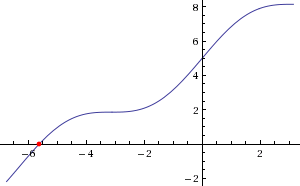
\includegraphics[scale=0.5]{plot_fx.png}
\end{center}

$$g(x) = 1 + \frac{1}{x + 1}$$

\begin{center}
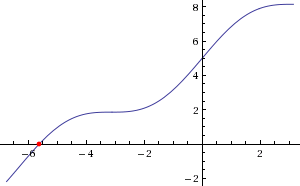
\includegraphics[scale=0.5]{plot_gx.png}
\end{center}

$$h(x) = \left(
\begin{array}{c}
-1 + x^2 + y^2 - \cos{x}\sin{y}\\
xy - \cos{y} - \sin{x}
\end{array}
\right)$$

\begin{center}
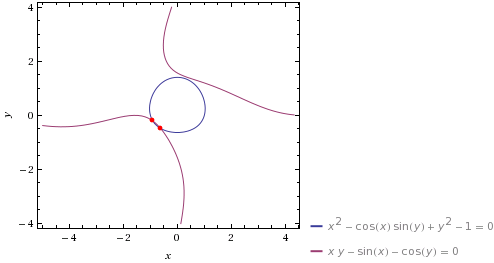
\includegraphics[scale=0.5]{plot_hx.png}
\end{center}

$$i(x) = \left(
\begin{array}{c}
x^2 + y - 10\\
x - y + 4
\end{array}
\right)$$

\begin{center}
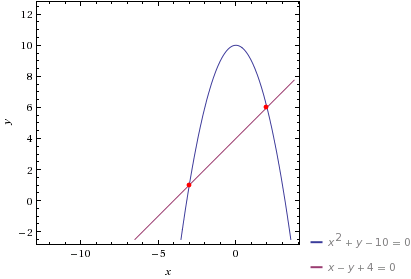
\includegraphics[scale=0.5]{plot_ix.png}
\end{center}

\subsection{S/I probak}

Hasteko, konfigurazio fitxategiaren irakurlea ondo dabilela ziurtatuko dugu. Beste probetan jada probatuko da konfigurazio sintaxi egokia, beraz, hemen sintaxi erroreak detektatzen dituela ziurtatuko da.

\paragraph{Fitxategi hutsa}

\begin{verbatim}
[x] Ez da aurkitu dimentsioa.
[x] Ezin izan da konfigurazio fitxategia ondo irakurri.
\end{verbatim}

\paragraph{Dimensio desegokia}

\begin{verbatim}
dimentsioa 0
\end{verbatim}

\begin{verbatim}
[x] Dimentsioak zero baina handiagoa izan behar du.
[?] LERROA: dimentsioa 0
[x] Ezin izan da konfigurazio fitxategia ondo irakurri.
\end{verbatim}

\begin{verbatim}
dimentsioa
\end{verbatim}

\begin{verbatim}
[x] Sintaxi desegokia dimentsioa emateko lerroan.
[?] LERROA: dimentsioa
[x] Ezin izan da konfigurazio fitxategia ondo irakurri.
\end{verbatim}

\paragraph{X0-ren tamaina desegokia}

\begin{verbatim}
dimentsioa 2
0.5
\end{verbatim}

\begin{verbatim}
[x] Dimentsioa eta X0-ren tamaina ez datoz bat.
[x] Ezin izan da konfigurazio fitxategia ondo irakurri.
[?] DIMENTSIOA: 2
[?] TAMAINA: 1
\end{verbatim}

\begin{verbatim}
dimentsioa 2
0.5
0.5
0.5
\end{verbatim}

\begin{verbatim}
[x] X0-ren elementu kopurura dimentsioa baina handiagoa da.
[x] Ezin izan da konfigurazio fitxategia ondo irakurri.
[?] DIMENTSIOA: 2
\end{verbatim}

\paragraph{Aukera desegokiak}

\subsection{Proba orokorrak}

Sekzio honetan $f(x)$, $g(x)$, $h(x)$ eta $i(x)$ funtzioak probatuko ditugu lehenetsitako aukerekin.

\subsection{Aukeren probak}

\end{document}